\chapter{Introduction}


% \emph{}

\section{Problem Statement and Approach}

Data undeniably plays a critical role in driving companies, especially in rapidly evolving business environments. Data offers insights that can solve problems, lead to improvements, help in making informed decisions, understand customer preferences, enhance marketing strategies, reduce costs, manage risks, and much more. Relying solely on specialists to retrieve data efficiently can be costly and time-consuming. Therefore, creating a query support tool that assists users in retrieving data from databases efficiently would be highly beneficial for fast-growing travel technology companies like Agoda.

At Agoda, the majority of employees are non-IT employees, which poses a challenge when retrieving important data. These employees often need to construct query statements, leading to inefficiencies in their workflow. They must either invest time in learning SQL or wait for the support team to respond to their query-related tickets, which can delay decision-making and reduce overall productivity.

This project aims to simplify data access and enhance productivity by enabling employees, especially non-technical users, to retrieve information without requiring SQL expertise. The Query Assistance tool leverages advanced technologies, including Large Language Models (LLMs) and LangChain, to provide comprehensive query support. It can fix incorrect queries, optimize performance, convert database syntax, and generate SQL statements from natural language input.

Initially, the tool will be developed as an API platform, allowing integration with various systems. In its later phase, it will be embedded into Superset to assist users directly within SQL Lab, streamlining workflows and reducing dependence on support teams. The integration with OpenMetadata enhances its capabilities, enabling the tool to analyze metadata and intelligently select the appropriate tables and columns for query construction. By combining these features, the Query Assistance tool addresses inefficiencies in query handling, helping organizations like Agoda save time, reduce costs, and improve decision-making processes.

\section{Objectives}
1.2.1 	To enhance correctness and increase efficiency in construction of queries.

1.2.2 	To develop API endpoints leveraging LLM services capable of fixing, converting, optimizing, and constructing queries.

1.2.3	To integrate Query Assistance with Agoda's existing services and tools, such as Superset and Slack,

\section{Scope of Work}
1.3.1	The API service to help solving SQL queries statement problems.

1.3.2	Develop capabilities for error handling in queries, ensuring syntax accuracy across multiple databases and correcting column and table names.

1.3.3	Implement query optimization techniques, utilizing partition columns to enhance performance and reduce both memory consumption and query execution time.

1.3.4	Build a module for translating natural language inputs into SQL query language.

1.3.5	Query Assist will only utilize data from Agoda Services to answer queries.

1.3.6	Query Assist will be integrated with Superset, Slack, and web-based platforms.

\section{Phases}
This project will be divided into three phases. The first phase focuses on error handling to ensure that we ultimately provide the correct query for the user. This includes correcting all syntax errors, accommodating syntax differences across databases, and fixing column names, table names, and typos in the query. The second phase focuses on optimizing the query such as using the partition column, decreasing memory consumption, and reducing the query execution time. The third and final phase aims to translate natural language into SQL query language.

\section{Task and Schedule}
    \subsection{Semester 1}
    % % \documentclass{article}
% \usepackage{pgfgantt}
% \usepackage{xcolor}

% \begin{document}

% Define custom colors
\definecolor{all}{RGB}{255,165,0} % Orange
\definecolor{shayathip}{RGB}{0,0,255} % Blue
\definecolor{ramin}{RGB}{0,128,0} % Green

\begin{ganttchart}[
    hgrid, vgrid,
    x unit=0.5cm, y unit title=0.8cm, y unit chart=0.6cm,
    time slot format=isodate-yearmonth,
    title/.append style={draw=none, fill=none},
    title label font=\bfseries\footnotesize,
    title label anchor/.append style={below=-1.6ex},
    bar/.append style={draw=none, fill=all},
    bar incomplete/.append style={fill=shayathip},
    bar progress label font=\footnotesize\bfseries,
    bar label font=\footnotesize,
    milestone label font=\footnotesize\bfseries,
    group label font=\bfseries\footnotesize,
    link/.style={-latex}
]{2025-08}{2025-12}

% Title row
\gantttitle{Phase}{1}
\gantttitle{Task}{1}
\gantttitle{August}{4}
\gantttitle{September}{4}
\gantttitle{October}{4}
\gantttitle{November}{4}
\gantttitle{December}{4} \\

% Phase 1
\ganttgroup{Phase 1}{2025-08}{2025-12}

% Tasks
\ganttbar[bar/.append style={fill=all}]{Project Discussion with company}{2025-08-01}{2025-08-04}
\ganttbar[bar/.append style={fill=all}]{Project Idea}{2025-08-01}{2025-08-04}
\ganttbar[bar/.append style={fill=all}]{Project Brainstorm}{2025-08-01}{2025-08-04}
\ganttbar[bar/.append style={fill=all}]{Design architecture design for project}{2025-08-01}{2025-08-04}
\ganttbar[bar/.append style={fill=shayathip}]{Set up project}{2025-08-01}{2025-08-04}
\ganttbar[bar/.append style={fill=shayathip}]{Design sequence diagram for create API to add and update Table details}{2025-08-01}{2025-08-04}
\ganttbar[bar/.append style={fill=shayathip}]{Implement query assist table details API}{2025-08-01}{2025-09-04}
\ganttbar[bar/.append style={fill=ramin}]{Design sequence diagram for tools in Query Assist}{2025-09-01}{2025-09-04}
\ganttbar[bar/.append style={fill=ramin}]{Implement tools for Query Assist}{2025-09-01}{2025-10-04}
\ganttbar[bar/.append style={fill=shayathip}]{Merge and Debug}{2025-10-01}{2025-10-04}
\ganttbar[bar/.append style={fill=shayathip}]{Prompt Tuning \& Monitor result}{2025-10-01}{2025-10-04}
\ganttbar[bar/.append style={fill=ramin}]{CI/CD + Deploy}{2025-10-01}{2025-10-04}
\ganttbar[bar/.append style={fill=ramin}]{Slack Integration}{2025-10-01}{2025-11-04}




% Phase 2.5
\ganttgroup{Phase 2.5}{2025-12}{2025-12}
\ganttbar[bar/.append style={fill=ramin}]{Merge PostgreSQL of V1 and V2}{2025-12-01}{2025-12-04}
\ganttbar[bar/.append style={fill=ramin}]{Merge code of V1 and V2}{2025-12-01}{2025-12-04}

% Phase 2
\ganttgroup{Phase 2}{2025-12}{2025-12}
\ganttbar[bar/.append style={fill=all}]{POC and Design the Phase 2 function}{2025-12-01}{2025-12-04}
\ganttbar[bar/.append style={fill=shayathip}]{Implement Optimization function}{2025-12-01}{2025-12-04}

\end{ganttchart}

% \end{document}

    \begin{table}[H]
        \centering
        \caption{Schedule of Semester 1}\label{tbl:schedule}
        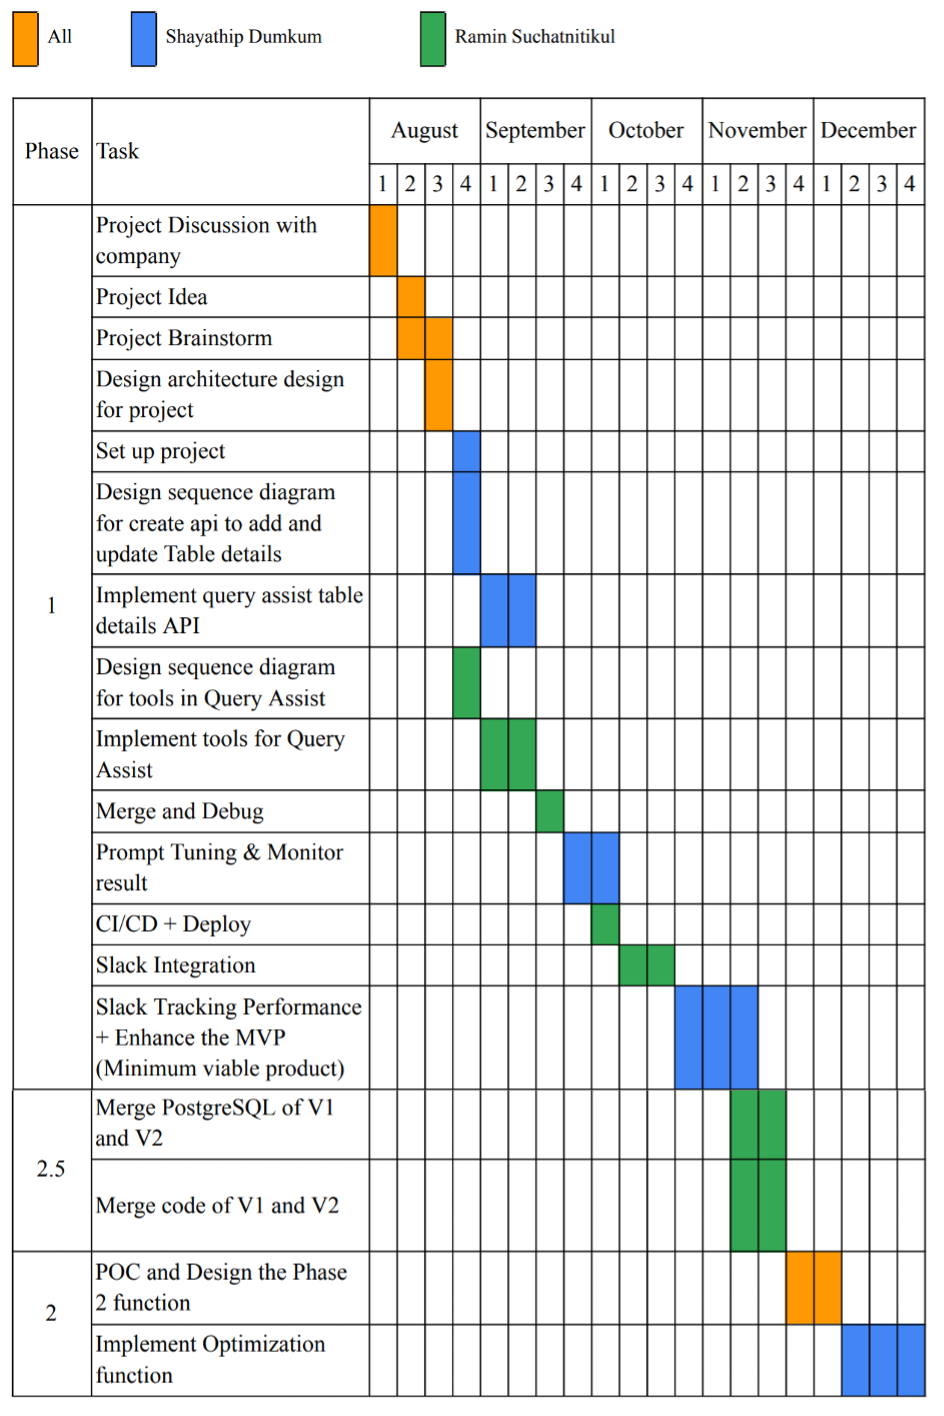
\includegraphics[width=15cm]{chapters/1/figures/plan.png}
    \end{table}

    % \begin{table}[H]
    %     \centering
    %     \caption{Gantt Chart for Query Assist Project}
    %     \label{tbl:gantt-chart}
    %     \begin{tabular}{|p{1cm}|p{5cm}|*{20}{c|}}
    %         \hline
    %         \textbf{Phase} & \textbf{Task} & \multicolumn{4}{c|}{\textbf{August}} & \multicolumn{4}{c|}{\textbf{September}} & \multicolumn{4}{c|}{\textbf{October}} & \multicolumn{4}{c|}{\textbf{November}} & \multicolumn{4}{c|}{\textbf{December}} \\
    %         \hline
    %         & & 1 & 2 & 3 & 4 & 1 & 2 & 3 & 4 & 1 & 2 & 3 & 4 & 1 & 2 & 3 & 4 & 1 & 2 & 3 & 4 \\
    %         \hline
    %         1 & Project Discussion with company & \cellcolor{orange} & \cellcolor{orange} & \cellcolor{orange} & \cellcolor{orange} & & & & & & & & & & & & & & & & \\
    %         \hline
    %         1 & Project Idea & \cellcolor{orange} & \cellcolor{orange} & \cellcolor{orange} & \cellcolor{orange} & & & & & & & & & & & & & & & & \\
    %         \hline
    %         1 & Project Brainstorm & \cellcolor{orange} & \cellcolor{orange} & \cellcolor{orange} & \cellcolor{orange} & & & & & & & & & & & & & & & & \\
    %         \hline
    %         1 & Design architecture design for project & \cellcolor{orange} & \cellcolor{orange} & \cellcolor{orange} & \cellcolor{orange} & & & & & & & & & & & & & & & & \\
    %         \hline
    %         1 & Set up project & & & & & \cellcolor{blue} & \cellcolor{blue} & \cellcolor{blue} & \cellcolor{blue} & & & & & & & & & & & & \\
    %         \hline
    %         1 & Design sequence diagram for create API to add and update Table details & & & & & \cellcolor{blue} & \cellcolor{blue} & \cellcolor{blue} & \cellcolor{blue} & & & & & & & & & & & & \\
    %         \hline
    %         1 & Implement query assist table details API & & & & & \cellcolor{blue} & \cellcolor{blue} & \cellcolor{blue} & \cellcolor{blue} & & & & & & & & & & & & \\
    %         \hline
    %         1 & Design sequence diagram for tools in Query Assist & & & & & & & & & \cellcolor{green} & \cellcolor{green} & \cellcolor{green} & \cellcolor{green} & & & & & & & & \\
    %         \hline
    %         1 & Implement tools for Query Assist & & & & & & & & & \cellcolor{green} & \cellcolor{green} & \cellcolor{green} & \cellcolor{green} & & & & & & & & \\
    %         \hline
    %         1 & Merge and Debug & & & & & & & & & & & & & \cellcolor{blue} & \cellcolor{blue} & \cellcolor{blue} & \cellcolor{blue} & & & & \\
    %         \hline
    %         1 & Prompt Tuning \& Monitor result & & & & & & & & & & & & & \cellcolor{blue} & \cellcolor{blue} & \cellcolor{blue} & \cellcolor{blue} & & & & \\
    %         1 & CI/CD + Deploy & & & & & & & & & & & & & \cellcolor{green} & \cellcolor{green} & \cellcolor{green} & \cellcolor{green} & & & & \\
    %         \hline
    %         1 & Slack Integration & & & & & & & & & & & & & & & & & \cellcolor{green} & \cellcolor{green} & \cellcolor{green} & \cellcolor{green} \\
    %         \hline
    %         1 & Slack Tracking Performance + Enhance the MVP (Minimum viable product) & & & & & & & & & & & & & & & & & \cellcolor{blue} & \cellcolor{blue} & \cellcolor{blue} & \cellcolor{blue} \\
    %         \hline
    %         2.5 & Merge PostgreSQL of V1 and V2 & & & & & & & & & & & & & & & & & & & \cellcolor{green} & \cellcolor{green} \\
    %         \hline
    %         2.5 & Merge code of V1 and V2 & & & & & & & & & & & & & & & & & & & \cellcolor{green} & \cellcolor{green} \\
    %         \hline
    %         2 & POC and Design the Phase 2 function & & & & & & & & & & & & & & & & & \cellcolor{orange} & \cellcolor{orange} & & \\
    %         \hline
    %         2 & Implement Optimization function & & & & & & & & & & & & & & & & & & \cellcolor{blue} & \cellcolor{blue} & \\
    %         \hline
    %     \end{tabular}
    % \end{table}

    \textbf{Task breakdown}
    \begin{table}[H]
        \centering
        \caption{Task Breakdown for Query Assist Project Semester 1}
        \label{tbl:task-breakdown}
        \begin{tabular}{|p{4cm}|p{10cm}|}
            \hline
            \textbf{Task} & \textbf{Description} \\
            \hline
            Project Discussion with company & Discuss the problem and scope of the project with the team in the company. \\
            \hline
            Project Idea & Research about the solution of the problem and study about LLMs. \\
            \hline
            Project Brainstorm & Gather ideas and brainstorming for one final solution. \\
            \hline
            Design architecture design for project & Drawing architecture diagram, sequence diagram, and use-case diagram of the Query Assist. \\
            \hline
            Set up project & Initiate the base structure code of the Query Assist project. \\
            \hline
            Design sequence diagram for create API to add and update Table details & Draw the sequence diagram for an API route to update information of tables and columns for Query Assist. \\
            \hline
            Implement query assist table details API & Implement the API route to update the tables and columns data following the metadata in OpenMetadata. \\
            \hline
            Design sequence diagram for tools in Query Assist & Draw sequence diagrams for tools that agents use. \\
            \hline
            Implement tools for Query Assist & Code custom functions for agents to use as tools to handle query problems. \\
            \hline
            Merge and Debug & Merge the Query Assist and API update functionalities. Debug the merged code. \\
            \hline
            Prompt Tuning \& Monitor result & Perform prompt tuning and monitoring to find practical prompts that solve query-related problems effectively. \\
            \hline
            CI/CD + Deploy & Implement CI/CD for the project using GitLab CI and deploy the Minimum Viable Product (MVP) for team testing. \\
            \hline
            Slack Integration & Integrate Query Assist with Slack to optimize ticket handling and reduce time usage. \\
            \hline
            Slack Tracking Performance + Enhance the MVP (Minimum Viable Product) & Implement performance tracking for Query Assist via Slack bot. Monitor and enhance error handling over time. \\
            \hline
            Merge PostgreSQL of V1 and V2 & Merge the new Query Assist database with the old version and test its usability. \\
            \hline
            POC and Design the Phase 2 function & Research and design the approach for optimization handling in Query Assist's second phase. \\
            \hline
            Implement Optimization function & Implement the optimization feature into Query Assist. \\
            \hline
        \end{tabular}
    \end{table}
\pagebreak
    \subsection{Semester 2}
    \begin{table}[H]
        \centering
        \caption{Schedule of Semester 1}\label{tbl:schedule2}
        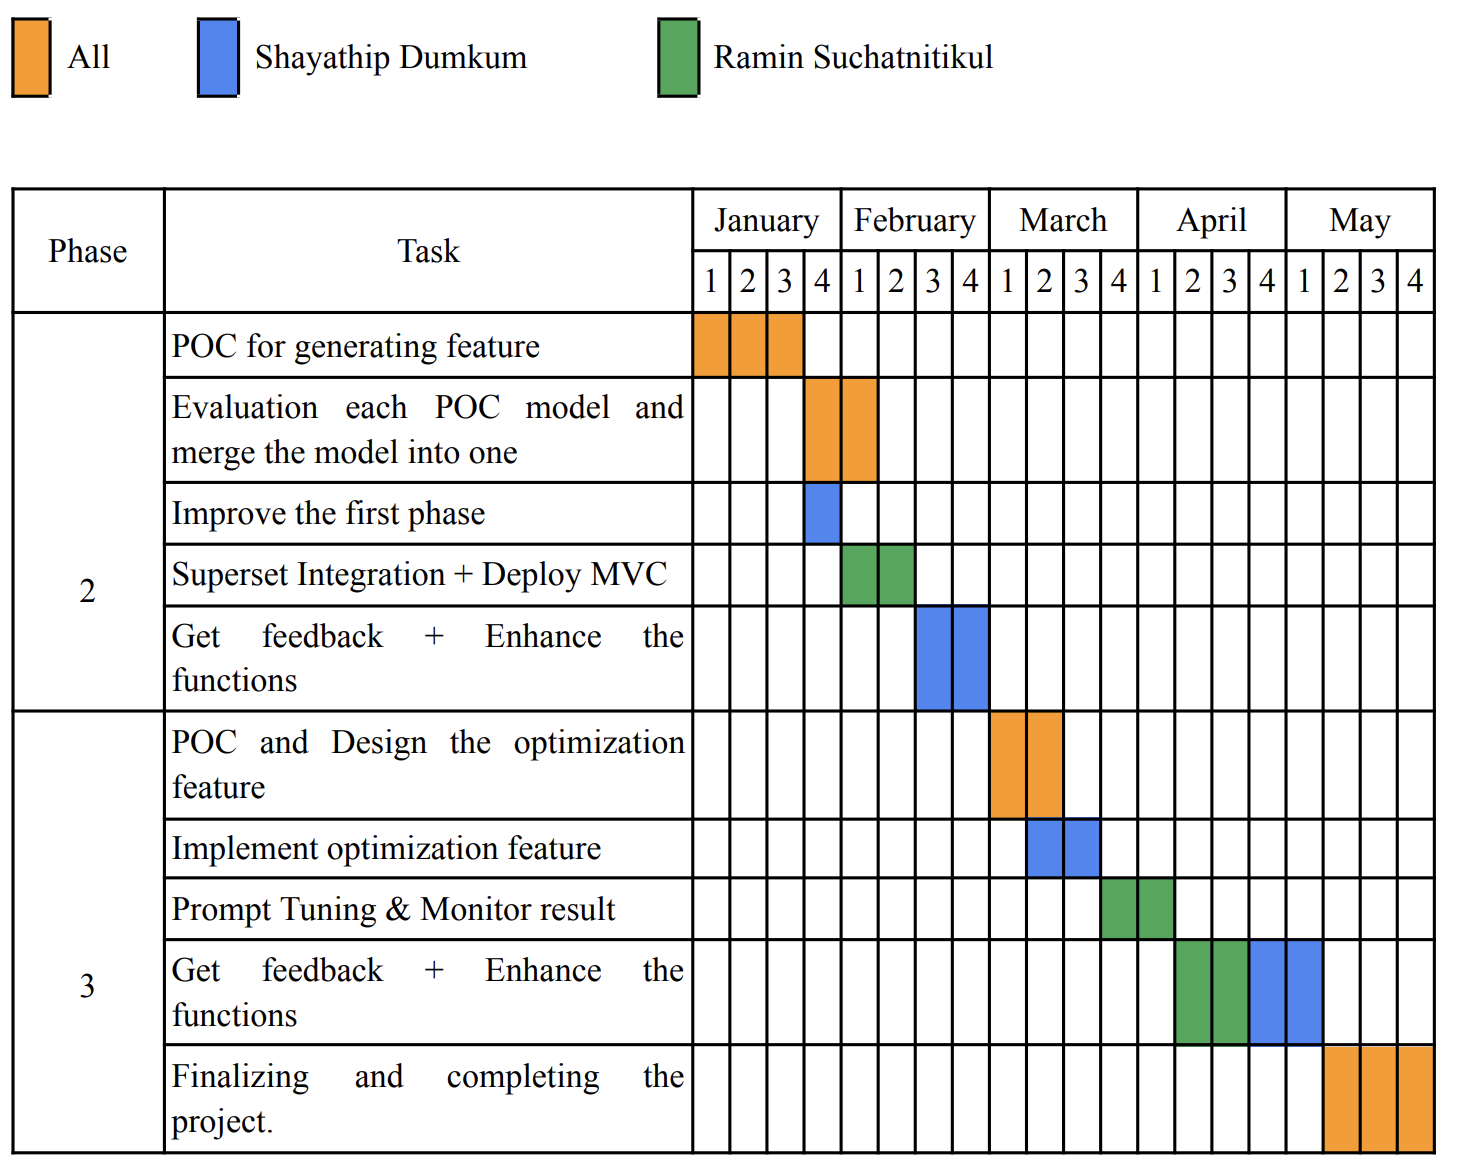
\includegraphics[width=15cm]{chapters/1/figures/plan2.png}
    \end{table}
    \textbf{Task breakdown}
    \begin{table}[!h]
        \centering
        \caption{Task Breakdown for Query Assist Project Semester 2}
        \label{tbl:task-breakdown2}
        \begin{tabular}{|p{4cm}|p{10cm}|}
            \hline
            \textbf{Task} & \textbf{Description} \\
            \hline
            POC for generating feature & Research and design the approach for constructing queries from the natural language feature of Query Assist. \\
            \hline
            Evaluation each POC model and merge the model into one & Evaluate the effectiveness of each solution and integrate them into a single comprehensive model. \\
            \hline
            Improve the first phase & Improve the first phase that has been launched based on feedback and its performance. \\
            \hline
            Superset Integration + Deploy MVC & Integrate Query Assist into Superset and deploy this version. \\
            \hline
            Get feedback + Enhance the functions & Get feedback from users and enhance project quality. \\
            \hline
            POC and Design the optimization feature & Implement optimization features into Query Assist. \\
            \hline
            Implement optimization feature & Tune prompts and monitor results for optimization features. \\
            \hline
            Prompt Tuning \& Monitor result & Tune prompts and monitor results for optimization features. \\
            \hline
            Get feedback + Enhance the functions & Get feedback from users and enhance project quality. \\
            \hline
            Finalizing and completing the project & Finalize the project and wrap up. \\
            \hline
        \end{tabular}
    \end{table}
\pagebreak

\section{Expected Outcomes}
The end goal of the project is to develop a comprehensive Query Assist tool that enables users to efficiently retrieve and manage data without needing SQL expertise. Key features include automated error correction, performance optimization, and the ability to translate natural language into SQL queries, all integrated into platforms like Slack and Superset, fostering enhanced data access and decision-making capabilities.

\textbf{Semester 1}
\begin{itemize}
    \item  Overall system design
    \begin{itemize}
        \item Architecture Design
        \item Use Case Diagram
        \item Sequence Diagram
        \item Flow Chart
    \end{itemize}

    \item  Query Assist Phase 1
    \begin{itemize}
        \item Correcting all syntax errors
        \item Accommodating syntax differences across databases
        \item Fixing typos in column names, and table names
    \end{itemize}

    \item  Integrate into Slack
    \item Deploy MVC (Minimum viable product)
\end{itemize}
\pagebreak
\textbf{Semester 2}
\begin{itemize}
    \item  Performance Metrics

    \item  Query Assist Phase 2
    \begin{itemize}
        \item Translate natural language to SQL query
    \end{itemize}

    \item Query Assist Phase 3
    \begin{itemize}
        \item Auto add partition column
        \item Decreasing memory consumption
        \item Reducing the query execution time
    \end{itemize}
\end{itemize}
\pagebreak
